%%%%%%%%%%%%%%%%%%%%%%%%%%%%%%%%%%%%%%%%%%%%%%%%%%%%%%%%%%%%%%%%%%%%%%%%%%%%%%%%
%2345678901234567890123456789012345678901234567890123456789012345678901234567890
%        1         2         3         4         5         6         7         8

\documentclass[letterpaper, 10 pt, conference]{ieeeconf}
% Comment this line out if you need a4paper

%\documentclass[a4paper, 10pt, conference]{ieeeconf}
% Use this line for a4 paper

\IEEEoverridecommandlockouts
% This command is only needed if
% you want to use the \thanks command

\overrideIEEEmargins
% Needed to meet printer requirements.

%In case you encounter the following error:
%Error 1010 The PDF file may be corrupt (unable to open PDF file) OR
%Error 1000 An error occurred while parsing a contents stream. Unable to analyze the PDF file.
%This is a known problem with pdfLaTeX conversion filter. The file cannot be opened with acrobat reader
%Please use one of the alternatives below to circumvent this error by uncommenting one or the other
%\pdfobjcompresslevel=0
%\pdfminorversion=4

% See the \addtolength command later in the file to balance the column lengths
% on the last page of the document

% The following packages can be found on http:\\www.ctan.org
\usepackage{graphics} % for pdf, bitmapped graphics files
\usepackage{epsfig} % for postscript graphics files
\usepackage{mathptmx} % assumes new font selection scheme installed
\usepackage{times} % assumes new font selection scheme installed
\usepackage{amsmath} % assumes amsmath package installed
\usepackage{newtxtext, newtxmath}
\usepackage{verbatim}
\usepackage{slashbox}
\usepackage{colortbl}
\definecolor{mygray}{gray}{.9}

\title{\LARGE \bf
ELEC6229: Receding Horizon Method
%\& Symposia*
}

\author{Zhikun Zhu, ID: 29356822% <-this % stops a space
%\begin{comment}
  % <-this % stops a space
}
%\end{comment}


\begin{document}



\maketitle
\thispagestyle{empty}
\pagestyle{empty}


%%%%%%%%%%%%%%%%%%%%%%%%%%%%%%%%%%%%%%%%%%%%%%%%%%%%%%%%%%%%%%%%%%%%%%%%%%%%%%%%
\begin{abstract}
  This report summarizes the implementation of receding horizon method and discusses the paramater choosing for control and prediction horizons.
\end{abstract}


%%%%%%%%%%%%%%%%%%%%%%%%%%%%%%%%%%%%%%%%%%%%%%%%%%%%%%%%%%%%%%%%%%%%%%%%%%%%%%%%


\section{Introduction of system model}
In this coursework, we are required to manage a super apple market on Mars using Receding Horizon Control (RHC), and we are demanded to minimize the cost within a 52 weeks period. The specifications of the problem is given by:
\begin{itemize}
  \item The total time period is 52 weeks.
  \item The re-order number \textbf{r} is fixed to be the choice in coursework 1 where $r=1$.
  \item The penalty for short stock (demand excess stock) is 20 coins per week and the warehouse cost is 5 coins per unit per week (pupw). At the end of the period, we will be charged 10 coins per unit apple to return them to earth.
  \item The order number \textbf{y} is flexible and to be determined by RHC.
\end{itemize}
For the convenience of analysis. For the range $1 \leq k \leq 52, k \in N^+$,  define the stock at the beginning of week $k$ is $z_k^-$ and at the end of the week $k$ is $z_k^+$. The demand $x_k$ and the order number $y_k$. The system model then becomes:
\begin{eqnarray}
      z_k^- &=& z_{k-1}^+ + y_{k-1}  \\
      z_k^+ &=& \max(z_k^- - x_k,0)
\end{eqnarray}

The weekly consumption of super apple on Mars is a random variable (RV) with following distribution:
\begin{table}[h]
  \caption{Apple consumption PDF}
  \label{consumptionPDF}
  \begin{center}
    \begin{tabular}{|c||c|c|c|c|c|c|c|}
      \hline
      Demand (x)   & 0 & 1 & 2 & 3 & 4 & 5 & 6\\
      \hline
      probability (p) & 0.04 & 0.08 & 0.28 & 0.4 & 0.16 & 0.02 & 0.02\\
      \hline
    \end{tabular}
  \end{center}
\end{table}

The weekly consumption is generated using rejection method, which principle has been introduced in the former coursework.

Following is the organization of remaining sections: in section \uppercase\expandafter{\romannumeral2}, the initial analysis of the reasonable choice of $y$ will be discussed before simulation. Section \uppercase\expandafter{\romannumeral3} promotes the optimal choice of $y$ from the perspective of RHC. Section \uppercase\expandafter{\romannumeral4} discussed parameters adjustments of RHC.  Section \uppercase\expandafter{\romannumeral5} conclude the work and evaluate the performance of RHC.


\section{Analysis before simulation}
According to Table. \ref{consumptionPDF}, the expectation of weekly consumption is $E(p_D(x)) = \sum \limits_{x=0}^6 p_D(x) \cdot x = 2.7$. Then, from the perspective of probability theory, the optimal solution is that at the beginning of each week, the stock is $2.7$ units. Since the choice of order number $y$ need to be an integer. Then, the suboptimal choice is maintaining the stock at $3$ at the beginning of each week.

According to the system model which described in section \uppercase\expandafter{\romannumeral1}, we can only place an order when $r \leq 1$, then the choice of $y$ for each week $k$ should be:
\begin{equation}
  y_k =     \left\{
  \begin{array}{rcl}
    0  & \mbox{for} & r_{k}>1  \\
    2 & \mbox{for} & r_{k}=1 \\
    3  & \mbox{for} & r_{k}=0
  \end{array}\right.
\end{equation}

It should be mentioned that we place an order on the Friday of each week, then the order number $y_k$ for the week $k$ is aiming to maintain the stock for the week $k+1$.

\section{Receding Horizon Method implementation}

The basic idea of receding horizon method is to predict $N$ steps ahead of the system at time $k$ to minimize a cost function $J(y)$, which is a function of $Y = [{y_k, y_{k+1},...,y_{k+N-1}}]$ and $X=[{x_k, x_{k+1},...,x_{k+N-1}}]$. And assign the first input $y_k$ as the input to the system. For a specific sequence of Y, the cost function for the system specified in section \uppercase\expandafter{\romannumeral1} is:
\begin{small}
\begin{equation}
  \begin{array}{rcl}
    J_N(X,Y) &=&  \sum \limits_{i = k}^{k+N-1} 5\cdot \max\left(\left(z_i^+-x_i\right),0\right) \\
    &+& 20\cdot \delta\left(
    \max\left(\left(z_i^+-x_i+0.1\right),0\right)\right)
  \end{array}
\end{equation}
\end{small}
Here $0.1$ is added to guarantee that the the algorithm won't get penalty when the demand is equals the stock. Simultaneous Eq.1, Eq.2 and Eq.4, we can get the totall cost within the window for a specific set pair $X$, $Y$ before we reach the end of the period:
\begin{equation}
  \begin{array}{rcl}
    J_N(X,Y) = \sum \limits_{i = k}^{k+N-1} 5\cdot \max\left(\left(z_{i-1}^+
    + y_{i-1}-x_i\right),0\right) \\
    + 20\cdot \delta\left(\max\left(\left(z_{i-1}^+ + y_{i-1}-x_i+0.1\right),0\right)\right)
  \end{array}
\end{equation}

For each possible sequence of $Y$, we need to traverse the demand space. According to Table. \ref{consumptionPDF}, we have $7^N$ possible demand sequences where $N$ is the window size. Then the weighted cost for $Y$ is defined by:
\begin{equation}
    J_N(Y) = \sum \limits_{X \in \mathbb{X}} J_N(X,Y) \cdot p(X)
\end{equation}
Where $\mathbb{X}$ is the demand space. The probability $p(X)$ is used to weight the cost according to itself probability, and it can be calculated from Table. \ref{consumptionPDF}. For example, when $N = 3$, the probability for $Y = [3,3,3]$ is $p(Y) = 0.4^3 = 0.0064$.

When the prediction window contains the final week, the cost function should be different. Besides, according to my implementation, when the prediction window trying to go beyond the 52-the week, the window size will be reduced to guarantee the 52-the week is the final predict week.
\begin{equation}
  \begin{array}{rcl}
    J_N(X,Y) &=& \sum \limits_{i = k}^{k+N-1} 5\cdot \max\left(\left(z_{i-1}^+
    + y_{i-1}-x_i\right),0\right) \\
    &+& 20\cdot \delta\left(\max\left(\left(z_{i-1}^+ + y_{i-1}-x_i +0.1\right),0\right)\right) \\
    &+& 5\cdot \delta\left(i-52\right)\left(\max\left(\left(z_{i-1}^+ + y_{i-1}-x_i+0.1\right),0\right)\right)
  \end{array}
\end{equation}

From the concept of RHC, we need to determine the prediction horizon size and control horizon size, the window mentioned before is the former one. Here, for this specific task, the control horizon, which is the key parameter to decide the optimal input $y$, is chosen to be $N_C = 1$, since the whole process is a stochastic and non-Markov process. Then the optimal choice $\hat{y}_k$ for time $k$ is got by finding the total cost starting with
\begin{equation}
\hat{y}_k = \arg \min \limits_{y_i} \sum \limits_{y_k=y_i, Y \in \mathbb{Y}} J_N(Y) \quad y_i \in [0,6]
\end{equation}

The simulation results for $500$ runs is shown in Fig. \ref{ADS_4_Simu}. The mean cost over the 52-week-period is $377.24$, which is got by taking the average over $5000$ runs, and the standard deviation is $57.63$. Then according to the central limit theory, we are  $99.5\%$ sure that the total cost is within $[375.14, 379.34]$
\begin{figure}[thpb]
   \centering
   \framebox{\parbox{0.4\textwidth}{
   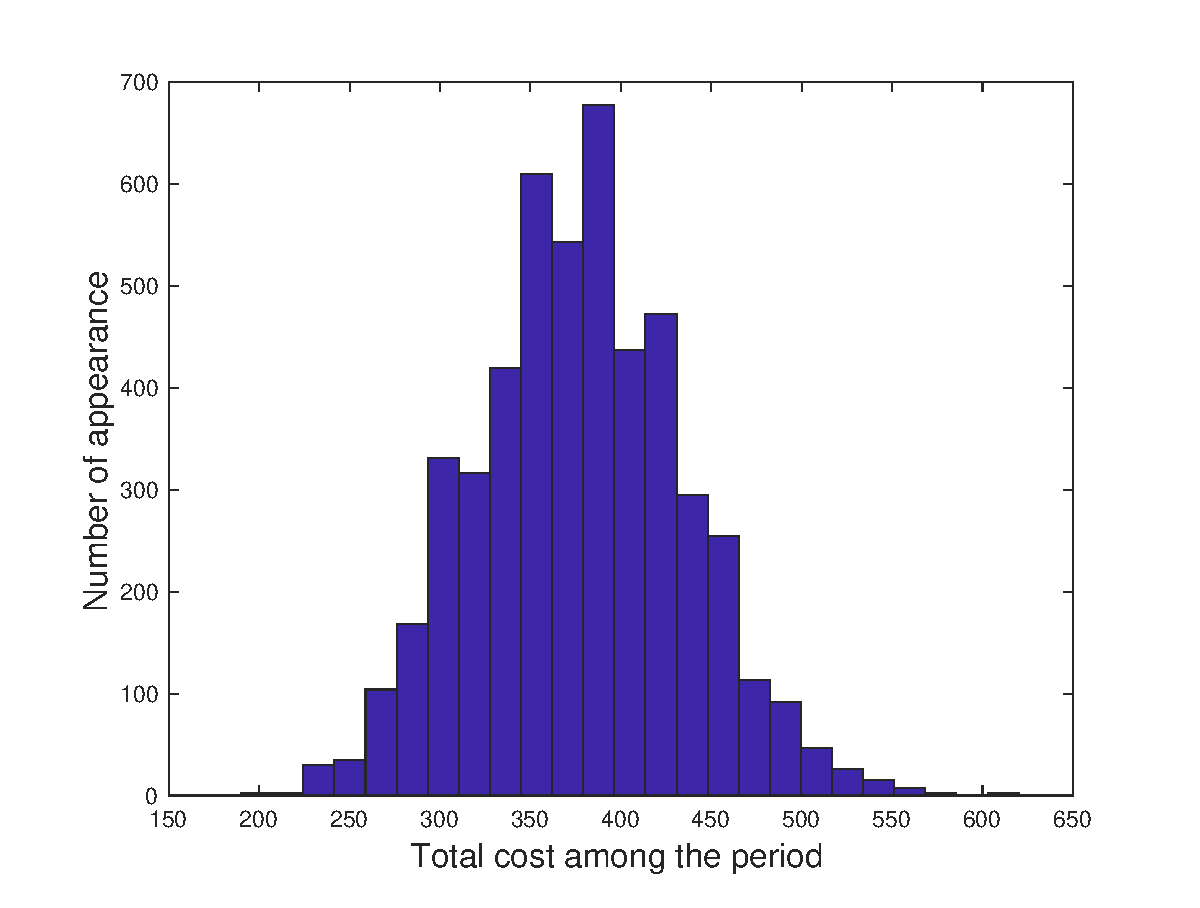
\includegraphics[width=0.4\textwidth]{ADS_4_Simu.eps}
   %\label{GBF_state}
}}
   %\includegraphics[scale=1.0]{figurefile}
   \caption{Cost simulation results for 500 times based on RHC.}
   \label{ADS_4_Simu}
\end{figure}

Table. \ref{52WeeksSimulation} shows the relationship between weekly stock and order number for that week. This result is identical to my analysis before simulation: maintaining the stock $z_k^- = 3$ all the time. Here the order number is range from $[1,6]$, since when $x_k^+ \geq 2$ we cannot order an apple, but when $x_k^+ \leq 1$, we do need to order some apple since the expectation of apple consumption is $2.7$.
\begin{table}[h]
  \caption{Simulation results for order number and stock}
  \label{52WeeksSimulation}
  \begin{center}
    \begin{tabular}{|c||c|c|c|c|c|c|c|c|c|c|}
      \hline
      \rowcolor{mygray}
      Week $k$  & 0   & 1 & 2 & 3 & 4 & 5 &6 &7 &8 &...\\
      \hline
      $x_k^+$  & 0       & 1 & 0 & 0 & 1 & 0 &3 &1 &2 &...\\
      \hline
      $y_k$ & 3       & 2 & 3 & 3 & 2 & 3  &0 &2 &1 &...\\
      \hline
      \rowcolor{mygray}
      Week $k$   &43 & 44   & 45 & 46 & 47 & 48 & 49 &50 &51  &52\\
      \hline
      $x_k^+$ & 0       & 0 & 0 & 0 & 1 & 1  &0 &1 &0 &0\\
      \hline
      $y_k$ & 3       & 3 & 3 & 3 & 2 & 2  &3 &2 &3 &End\\
      \hline
    \end{tabular}
  \end{center}
\end{table}

Inspecting Table. \ref{52WeeksSimulation}, we found that when $x_k^+ \geq 2$ the choice of $y_k = 1$. This is due to that $r$ is fixed to be 1, which means when $x_k^+ \geq 2$, the first week of in the prediction window will not order any apple no matter what order number we choose. Then, when $N_C = 1$, the costs specified in Eq.8 are the same for each $y_i$, then, the algorithm will choose $y_k$ to be the first element in the order space $[0,1,...,6]$ as $\hat{y}$, which is $1$.
\section{RHC parameters discussion}
The key parameters for RHC method are prediction horizon size $N_P$ and control horizon size $N_C$. The results got in last section is based on $N_P =3$ and $N_C=1$.

For this specific problem, I think the choice of $N_P$ has limited influence on the results. Because the process is stochastic, the demand for each week is an RV that we can only know its distribution and have no idea of what the real demand will be, then we cannot predict the real stock for the future. All our cost calculation (Eq.6) are based on probability, which will always choose to maintain $z_k^- =3$, which is only determined by $y_k$, $z_{k-1}^+ $, and irrelevant to the future order number. Thus extend $N_P$ will not improve the performance.

For the choice of $N_C$, it shares the same reason with the choice of $N_P$, since we have only the PDF of future demand, then, according to Eq.8, the algorithm tries to minimize the cost, but we only got the PDF of the demand, then, the optimal choice will be maintaining $z_k^- =3$ when $k$ is within the $N_P$ window, and choose $\hat{y}_k= 3$ when $k$ go beyond $N_P$.
\section{Conclusion and evaluation}
There are two way to implement Eq.6: Monte Carlo method or traverse all the possible $Y$ with respect probability. My implementation used the second method. However, Eq.6 can also be achieved approximately by Monte Carlo method, where we can randomly generate $N$ demand sequences $X_n \thicksim p(X)$. And the cost for each $Y$ is got based on these $X_n$.

Due to the low efficiency of generating apple consumption RVs, the Monte Carlo method expects more processing time than my implementation, which is a disadvantage. However, as $N_P$ increase, $p(Y)$ may cause floating overflow, I think this may be improved by using $\sum -\log(p(y_i))$ instead of $p(Y)$ as the weight.

Besides, from my perspective, $r=1$ limit the overall performance of the algorithm, since such parameter is optimal with fixed $y=3$, but here $y$ is flexible. The best choice $r$ is $2$, which guarantee the minimum stock $x_k^- = 3$ when $x_{k-1}^+ \leq 2$. I also simulated when $r=2$, where I have $99.95\%$ confidence the cost is in the range $[348.02, 360.90]$.

In conclusion, the RHC method is implemented to the system, which markedly minimzed the cost ($E(J) = 377.24$) compared to the result in the coursework \uppercase\expandafter{\romannumeral2} ($E(J) = 413.17$ ). And the relevant issues are properly discussed.
\addtolength{\textheight}{-12cm}
 % This command serves to balance the column lengths
% on the last page of the document manually. It shortens
                                  % the textheight of the last page by a suitable amount.
                                  % This command does not take effect until the next page
                                  % so it should come on the page before the last. Make
                                  % sure that you do not shorten the textheight too much.
%\bibliographystyle{ieeetr}
%\bibliography{cite}

\end{document}
